% // ============================================================================
%//
%// Copyright (c) 1999 The CGAL Consortium
%//
%// This software and related documentation is part of an INTERNAL release
%// of the Computational Geometry Algorithms Library (CGAL). It is not
%// intended for general use.
%//
%// ----------------------------------------------------------------------------
%//
%// release       :
%// release_date  :
%//
%// file          : /doc_tex/basic/Triangulation3/TDS3.tex
%// revision      : $Revision$
%//
%// author(s)     : Monique Teillaud <Monique.Teillaud@sophia.inria.fr>
%//
%// coordinator   : INRIA Sophia Antipolis (Mariette Yvinec <Mariette.Yvinec@sophia.inria.fr>)
%//
%//============================================================================
\chapter{Triangulation Data Structure in 3D}
\label{chapter-TDS3}

\section{Introduction}
\label{TDS3-sec-intro}

A three-dimensional triangulation is a three-dimensional simplicial
complex, pure connected and without singularities \cite{by-ag-98}. Its
cells ($3$-faces, tetrahedra) are such that two cells either do not
intersect or share a common facet ($2$-face), edge ($1$-face) or
vertex ($0$-face).

A geometric triangulation has two aspects: the combinatorial structure which
gives the incidence and adjacency relations between faces, and the
geometric information related to the position of vertices.

\cgal\ proposes 3D geometric triangulations in which these
two aspects are clearly separated.
As described in Chapter~\ref{chapter-Triangulation3}, a geometric
triangulation of a set of points in $\R^d$ is a partition of the
whole space $\R^d$ into cells having $d+1$ vertices: some of them
are infinite, they are obtained by linking an additional vertex at
infinity to each facet of the convex hull of the points.
The underlying combinatorial triangulation of such a triangulation
without boundary of $\R^d$ can be seen as a triangulation of the
topological sphere $S^d$ in $\R^{d+1}$. 

This chapter deals with 3D-triangulation data structures, meant to
maintain the combinatorial information for 3D-geometric
triangulations. The reader interested in geometric triangulations of
$\R^3$ is advised to read Chapter~\ref{chapter-Triangulation3}.

\subsection{Representation}
\label{TDS3-sec-def}

In \cgal, a triangulation data structure is a
container of cells ($3$-faces) and vertices ($0$-faces). Each cell gives
access to its four incident vertices and to its four adjacent
cells. Each vertex gives access to one of its incident cells.

The four vertices of a cell are indexed with 0, 1, 2 and 3.  The
neighbors of a cell are also indexed with 0, 1, 2, 3 
in such a way that the neighbor indexed by $i$ is opposite to the vertex
with the same index (see Figure~\ref{TDS3-fig-repres}).

\begin{ccTexOnly}
\begin{figure}
\begin{center} 
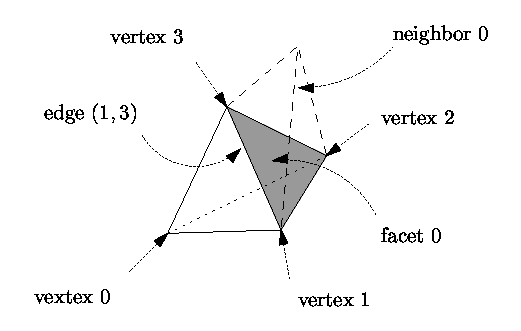
\includegraphics{repres.eps}
\end{center}
\caption{Representation \label{TDS3-fig-repres}}
\end{figure} 
\end{ccTexOnly}

\begin{ccHtmlOnly}
<img border=0 src="./repres.gif" align=center
alt="Representation">
\end{ccHtmlOnly}

Edges ($1$-faces) and facets ($2$-faces) are not explicitely
represented: a facet is given by a cell and an index (the facet
\ccc{i} of a cell \ccc{c} is the facet of \ccc{c} that is opposite to
the vertex of index \ccc{i}) and an edge is given by a cell and two
indices (the edge \ccc{(i,j)} of a cell \ccc{c} is the edge
whose endpoints are the vertices of indices \ccc{i} and \ccc{j} of
\ccc{c}). 

\subsection{Degenerate Dimensions}
\label{TDS3-sec-degen_dim}
As \cgal\ explicitely deals with all degenerate cases, a
3D-triangulation data structure in \cgal\ can handle the cases when
the dimension of the triangulation is lower than~3.

Thus, a 3D-triangulation data structure can store a triangulation of a
topological sphere $S^d$ of $\R^{d+1}$, for any $d \in \{-1,0,1,2,3\}$. 

Let us give, for each dimension, the example corresponding to the
triangulation data structure having a minimal number of vertices, i.e. a 
simplex. These examples are illustrated by presenting their usual
geometric embedding. 
\begin{itemize}
\item \emph{dimension 3.} The triangulation data structure consists of
the boundary of a 4-dimensional simplex, which has 5 vertices. A
geometric embedding consists in choosing one of these vertices to be
infinite, thus four of the five 3-cells become infinite: the geometric
triangulation has one finite tetrahedron remaining, each of its facets
being incident to an infinite cell. See Figure~\ref{TDS3-fig-topo-simplex4}.
\begin{ccTexOnly}
\begin{figure}
\begin{center} 
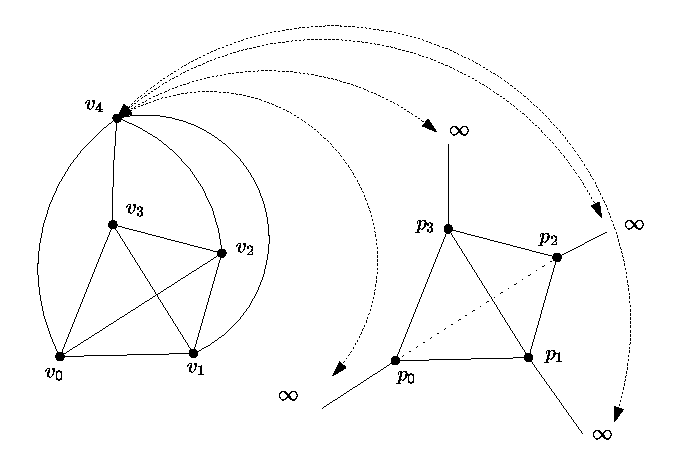
\includegraphics{topo-simplex4.eps}
\end{center}
\caption{4D simplex and a 3D geometric embedding \label{TDS3-fig-topo-simplex4}}
\end{figure} 
\end{ccTexOnly}
\begin{ccHtmlOnly}
<img border=0 src="./topo-simplex4.gif" align=center
alt="4D simplex and a 3D geometric embedding">
\end{ccHtmlOnly}
\item \emph{dimension 2.} We have 4 vertices forming one 3-dimensional
simplex, i.e. the boundary of a tetrahedron. The geometric embedding in
the plane consists in choosing one of these vertices to be infinite,
then the geometric triangulation has one finite triangle whose edges are
incident to the infinite triangles. See Figure~\ref{TDS3-fig-topo-simplex3}.
\begin{ccTexOnly}
\begin{figure}
\begin{center} 
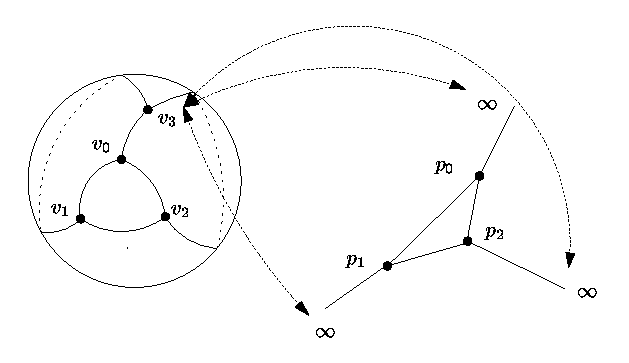
\includegraphics{topo-simplex3.eps}
\end{center}
\caption{3D simplex and a 2D geometric embedding \label{TDS3-fig-topo-simplex3}}
\end{figure} 
\end{ccTexOnly}
\begin{ccHtmlOnly}
<img border=0 src="./topo-simplex3.gif" align=center
alt="3D simplex and a 2D geometric embedding">
\end{ccHtmlOnly}
\item \emph{dimension 1.} A 2-dimensional simplex (a triangle) has 3
vertices. The geometric embedding is and edge whose vertices are linked
to an infinite point.  See Figure~\ref{TDS3-fig-topo-simplex2}.
\begin{ccTexOnly}
\begin{figure}
\begin{center} 
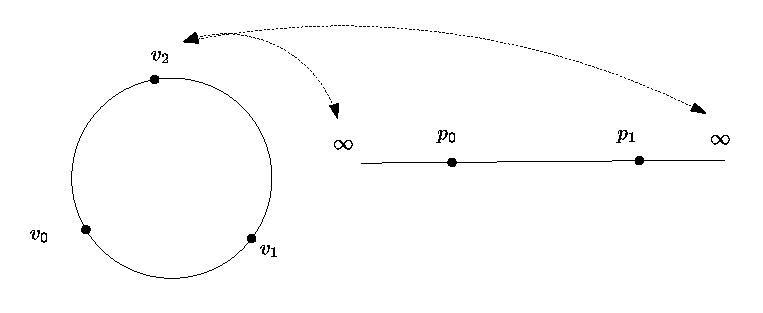
\includegraphics{topo-simplex2.eps}
\end{center}
\caption{2D simplex and a 1D geometric embedding \label{TDS3-fig-topo-simplex2}}
\end{figure} 
\end{ccTexOnly}
\begin{ccHtmlOnly}
<img border=0 src="./topo-simplex2.gif" align=center
alt="2D simplex and a 1D geometric embedding">
\end{ccHtmlOnly}
\end{itemize}

The last three cases are defined uniquely:
\begin{itemize}
\item \emph{dimension 0.} A 0-dimensional triangulation is
combinatorially equivalent to the boundary of a 1-dimensional simplex
(an edge), which consists of 2 vertices. One of them becomes infinite
in the geometric embedding, and there is only one finite vertex
remaining. The two vertices are adjacent.
\item \emph{dimension -1.} This dimension is a convention to represent a 
0-dimensional simplex, that is a sole vertex, which will be
geometrically embedded as an ``empty'' triangulation, only having one
infinite vertex.
\item \emph{dimension -2.} This is also a convention. The
triangulation data structure has no vertex. There is no associated
geometric triangulation.
\end{itemize} 

Note that the notion of infinite vertex has no meaning for the
triangulation data structure. The infinite vertex of the geometric
embedding is a vertex without any particularity in the
combinatorial triangulation.

The implicit representation of facets (resp. edges) still holds
for degenerate ($< 3$) dimensions : in dimension~2, each cell has only one
facet of index 3, and 3 edges $(0,1)$, $(1,2)$ and $(2,0)$; in
dimension~1, each cell has one edge $(0,1)$. 

\subsection{Validity}
\label{TDS3-sec-Valid}
A 3D combinatorial triangulation is said to be \ccc{locally valid} 
iff the following is true:

{\bf (a)} When a cell $c$ has a neighbor pointer to another cell $c'$,
then reciprocally this cell $c'$ has a neighbor pointer to $c$, and
$c$ and $c'$ have three vertices in common. These cells are called
adjacent. 
% Two adjacent cells have reciprocal neighbor pointers to each
% other and they have three vertices in common. 

{\bf (b)} The cells have a coherent orientation: if two cells $c_1$
and $c_2$ are adjacent and share a facet with vertices $u,v,w$, then
the vertices of $c_1$ are numbered $(v_0^1 = u, v_1^1 = v, v_2^1 = w,
v_3^1)$, and the vertices of $c_2$ are numbered $(v_0^2 = v, v_1^2 = u,
v_2^2 = w, v_3^2)$, up to positive permutations of $(0,1,2,3)$. In
other words, if we embed the triangulation in $\R^3$, then the fourth
vertices $v_3^1$ and $v_3^2$ of $c_1$ and $c_2$ see the common facet
in opposite orientations. See Figure~\ref{TDS3-fig-comborient}.

The set {\Large $\sigma$}$_4$ of permutations of
$(0,1,2,3)$ has cardinality 24, and the set of positive permutations
${\cal A}_4$ has cardinality 12. Thus, for a given orientation, there
are up to 12 different orderings of the four vertices of a cell. Note
that circular permutations are negative and so do not preserve the
orientation of a cell.

\begin{ccTexOnly}
\begin{figure}[htbp]

\begin{center} 
\includegraphics{comborient.eps} 
\end{center}
\caption{Coherent orientations of two cells (3-dimensional case)
\label{TDS3-fig-comborient}} 
\end{figure} 
\end{ccTexOnly}

\begin{ccHtmlOnly}
<img border=0 src="./comborient.gif" align=center alt="Orientation of a cell (3-dimensional case)">
\end{ccHtmlOnly}

The \ccc{is_valid()} method provided by \cgal\ checks the local
validity of a given triangulation data structure.
 
\section{Software Design}
\label{TDS3-sec-design}

The 3D- triangulation data structure class of \cgal\ is designed to be
used as a combinatorial layer for another class on an upper geometric
layer \cite{k-ddsps-98}. This upper class can be the 3D-Triangulation class of
\cgal. Figure~\ref{TDS3-fig-layers} shows the organization of the
software design in this case.

\begin{ccTexOnly}
\begin{figure}[htbp]

\begin{center} 
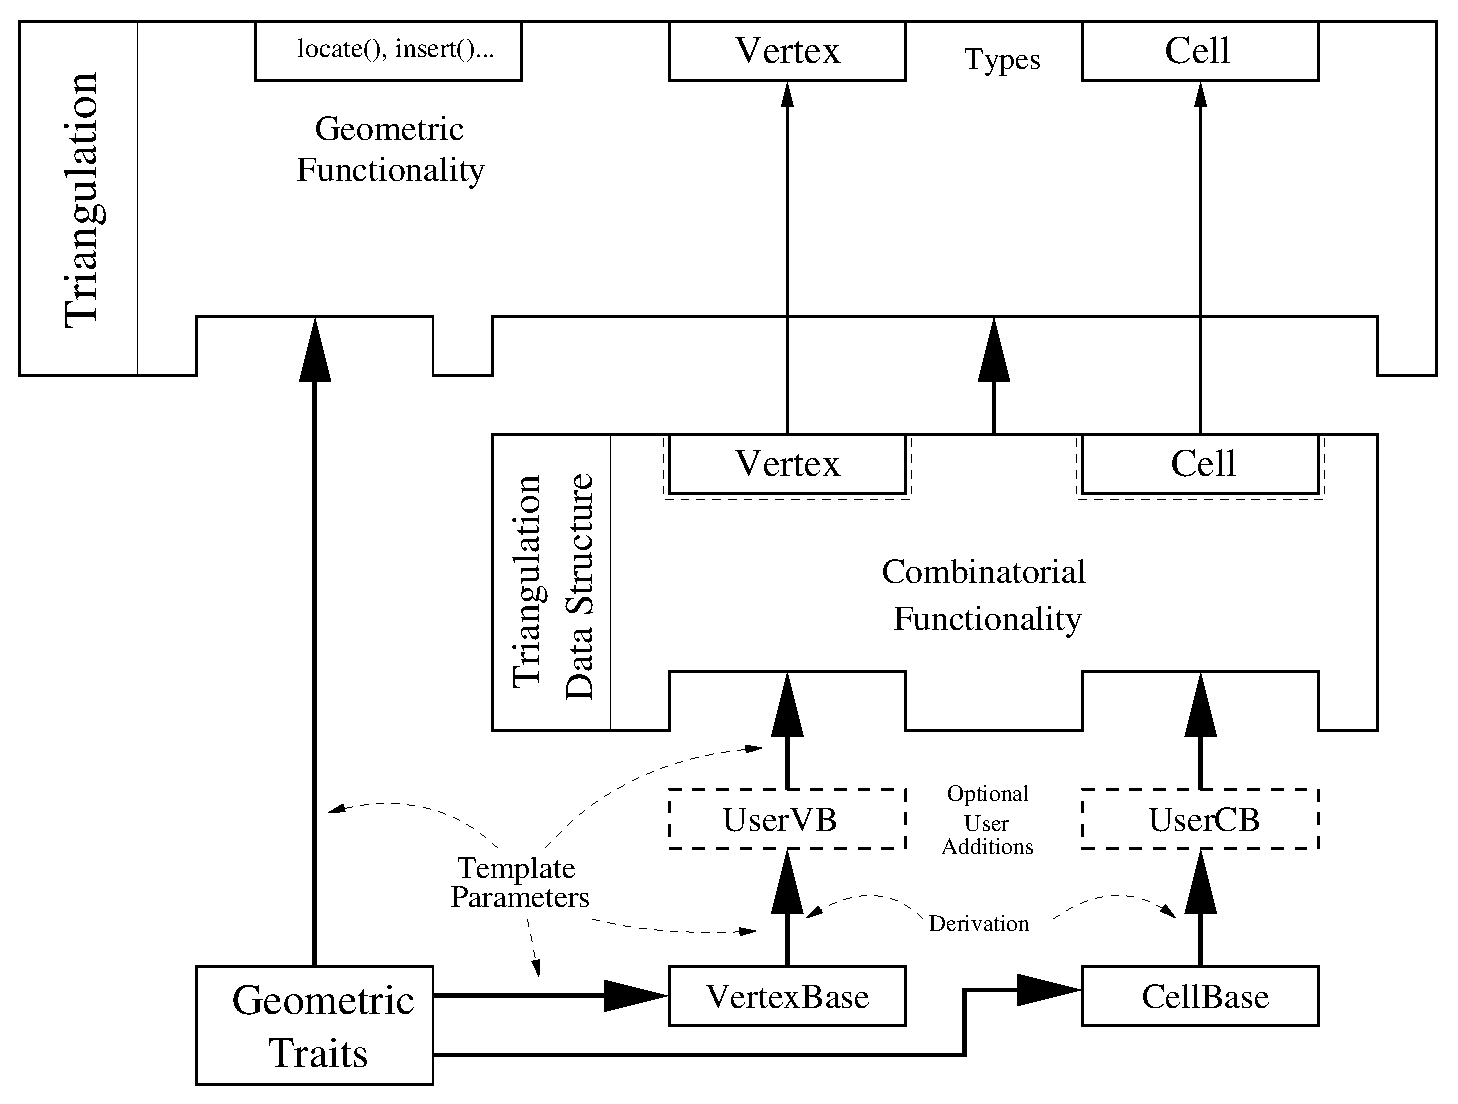
\includegraphics{design.eps} 
\end{center}
\caption{Layers in the software design\label{TDS3-fig-layers}} 
\end{figure} 
\end{ccTexOnly}

\begin{ccHtmlOnly}
<img border=0 src="./design.gif" align=center alt="Layers in the software design">
\end{ccHtmlOnly}

In the bottom layer, the \cgal\ base classes store elementary
geometric information.  These classes are parameterized by a geometric
traits class providing all the geometric types. A vertex has a pointer
to a cell, and a cell has four pointers to vertices. These pointers
are of type \ccc{void*}.

The middle layer class stores the triangulation data structure, which
is purely combinatorial. A vertex of the triangulation data structure
has a pointer to a cell of the triangulation data structure, and a
cell has four pointers to vertices. These pointers are usual
\ccc{C++} pointers. The triangulation data structure provides
operations such as insertion of a new vertex in a given cell, on a
$1$ or $2$-face. It also allows, if the dimension of the triangulation
is smaller than $3$, to insert a vertex so that the dimension of the
triangulation is increased by one. The triangulation data
structure is responsible for the combinatorial integrity of the
triangulation. 

It is up to the user to derive its own base classes from the \cgal\
base classes to add any other information he may need for his given
application, or to write his own base classes from scratch. In this
case, his base classes must be models for the concepts described in
Section~\ref{TDS3-sec-concept-Base}. As the triangulation data
structure class is parameterized by the base vertex and the base cell
classes. it will consider the user's bases classes instead of the
predefined base classes.

The upper layer, described in Chapter~\ref{chapter-Triangulation3}, is
the geometric triangulation class, providing operations such as
location of a point in the triangulation, insertion of a point, and is
responsible for the geometric validity. A vertex of the triangulation
has a pointer to a cell and a cell has four pointers to
vertices. These pointers are \cgal\ \emph{handles}. The triangulation
data structure class is one of the template parameters of the
geometric triangulation class. The user may choose to replace the
\cgal\ triangulation data structure class by its own triangulation
data structure, in this case, his class has to be a model of the
concept described in Section~\ref{TDS3-sec-concept}.

\section{Examples}
\label{TDS3-sec-examples}
The following example shows how to construct a 3D triangulation data
structure by inserting vertices.
\begin{verbatim}
#include <CGAL/basic.h>

#include <iostream>

#include <vector>

#include <CGAL/Cartesian.h>
#include <CGAL/Point_3.h>

#include <CGAL/Triangulation_geom_traits_3.h>
#include <CGAL/Triangulation_cell_base_3.h>
#include <CGAL/Triangulation_vertex_base_3.h>
#include <CGAL/Triangulation_data_structure_3.h>

// the definition of the geometric traits class is necessary to
// instanciate base vertices and cells but will in fact never be used
// in the program 
typedef CGAL::Cartesian<double>  Rep;
typedef CGAL::Triangulation_geom_traits_3<Rep> Gt;

typedef CGAL::Triangulation_vertex_base_3<Gt> Vb;
typedef CGAL::Triangulation_cell_base_3<Gt> Cb;

typedef CGAL::Triangulation_data_structure_3<Vb,Cb> Tds;

typedef typename Tds::Cell TDSCell;
typedef typename Tds::Vertex TDSVertex;

int main()
{
  Tds T;

  assert( T.number_of_vertices() == 0 );
  assert( T.dimension() == -2 );
  assert( T.is_valid() );

  std::vector<TDSVertex> V(5);
  std::vector<TDSVertex*> PV(7);

  PV[0] = T.insert_increase_dimension(V[0]);
  assert( T.number_of_vertices() == 1 );
  assert( T.dimension() == -1 );
  assert( T.is_valid() );

  int i;
  // each of the following insertions of vertices increases the dimension
  for ( i=1; i<5; i++ ) {
    PV[i] = T.insert_increase_dimension(V[i], PV[0]);
    assert( T.number_of_vertices() == i+1 );
    assert( T.dimension() == i-1 );
    assert( T.is_valid() );
  }
  assert( T.number_of_cells() == 5 );

  // we now have a simplex in dimension 4

  // cell incident to PV[0]
  TDSCell* c = PV[0]->cell();
  int ind;
  assert( c->has_vertex( PV[0], ind ) );
  // PV[0] is the vertex of index ind in c

  // insertion of a new vertex in the facet opposite to PV[0]
  PV[5] = T.insert_in_facet(TDSVertex(), c, ind);
  
  assert( T.number_of_vertices() == 6 );
  assert( T.dimension() == 3 );
  assert( T.is_valid() );

  // insertion of a new vertex in c
  PV[6] = T.insert_in_cell( TDSVertex(), c );

  assert( T.number_of_vertices() == 7 );
  assert( T.dimension() == 3 );
  assert( T.is_valid() );

  std::ofstream oFileT("output_tds",ios::out);
  // writing file output_tds; 
  oFileT << T; 

  return 0;
}
\end{verbatim}

\clearpage

\section{Concepts}

This section describes the concepts for a 3D- triangulation data
structure, its vertices and cells.

\subsection{Concepts for a 3D- Triangulation Data Structure}
\label{TDS3-sec-concept} 
\begin{ccClassTemplate}{Tds<Vb,Fb>}

The triangulation data structure must be able to represent a
triangulation of a topological sphere $S^d$ of $\R^{d+1}$, for $d \in
\{-1,0,1,2,3\}$.
The triangulation data structure must be templated by the base
vertex and the base cell classes. 
(see~\ref{TDS3-sec-intro})

\ccCreationVariable{tds}

A class \ccClassTemplateName\ that satisfies the requirements for a
triangulation data structure class must provide the following types and
operations. 

\ccTypes
\ccThree{typedef triple <Cell*, int, int>}{Facet }{}
\ccThreeToTwo

\ccNestedType{Vertex }{Vertex}
\ccGlue
\ccNestedType{Cell}{Cell type}
Requirements for \ccc{Vertex} and \ccc{Cell} are described in
Sections~\ref{TDS3-sec-concept-Tds_Vertex}
and~\ref{TDS3-sec-concept-Tds_Cell}.

\ccTypedef{typedef triple<Cell*, int, int> Edge;}{\ccc{(c,i,j)} is the
edge of cell \ccc{c} whose vertices indices are \ccc{i} and
\ccc{j}. (see Section~\ref{TDS3-sec-def})}
\ccGlue
\ccTypedef{typedef pair<Cell*, int>  Facet;}{\ccc{(c,i)} is the facet
of \ccc{c} opposite to the vertex of index \ccc{i}. (see
Section~\ref{TDS3-sec-def})} 


The following iterators allow to visit all the vertices, edges, facets
and cells of the triangulation data structure. They are all
bidirectional, non mutable iterators.

\ccNestedType{Cell_iterator}{}
\ccGlue
\ccNestedType{Facet_iterator}{}
\ccGlue
\ccNestedType{Edge_iterator}{}
\ccGlue
\ccNestedType{Vertex_iterator}{}

The following circulators allow us to visit all the cells and facets
incident to a given edge. They are bidirectional and non mutable.

\ccNestedType{Facet_circulator}{}
\ccGlue
\ccNestedType{Cell_circulator}{}

\ccCreation
\ccThree{Tds<Vb,Fb>}{tds.set_number_of_vertices()}{}

\ccConstructor{\ccClassName();}
{A default constructor.}

\ccConstructor{\ccClassName(const Tds & tds1);}
{Copy constructor. All the vertices and cells are duplicated.}

\ccMethod{Tds<Vb,Fb> operator=(const Tds & tds1);}
{Assignment. All the vertices and cells are duplicated.}

The previous first two methods are equivalent.

\ccMethod{void swap(Tds & tds1);} 
{Swaps \ccVar\ and \ccc{tds1}. There is no copy of cells and vertices,
thus this method runs in constant time. Should be preferred to
\ccVar=\ccc{tds1} or \ccVar(\ccc{tds1}) when \ccc{tds1} is deleted after
that.}

\ccMethod{Vertex* copy_tds(const Tds & tds1, Vertex* v = NULL);}
{\ccc{tds1} is copied into \ccVar. If $v != NULL$, the vertex of \ccVar\ 
corresponding to \ccc{v} is returned, otherwise \ccc{NULL} is returned.
\ccPrecond{The optional argument \ccc{v} is a vertex of \ccc{tds1}.}}

\ccFunction{void \ccTilde\ccVar();}
{Destructor. All vertices and cells are deleted, and \ccVar\ itself is
deleted.} 

\ccAccessFunctions

\ccMethod{int dimension() const;}
{The dimension of the topological sphere triangulated.}

\ccMethod{int number_of_vertices() const;}
{The number of vertices. Note that the triangulation data structure has one
more vertex than an associated geometric triangulation, since the
infinite vertex is a standard vertex and is thus also counted.}

\ccHeading{Non constant-time access functions}
\ccMethod{int number_of_cells() const;}
{The number of cells. Returns 0 if \ccVar.\ccc{dimension()}$<3$.}
\ccGlue
\ccMethod{int number_of_facets() const;}
{The number of facets. Returns 0 if \ccVar.\ccc{dimension()}$<2$.}
\ccGlue
\ccMethod{int number_of_edges() const;}
{The number of edges. Returns 0 if \ccVar.\ccc{dimension()}$<1$.}

\begin{ccAdvanced}
\ccHeading{Setting}
\ccMethod{void set_dimension(int n);}
{Sets the dimension to \ccc{n}.}

\ccMethod{void set_number_of_vertices(int n);}
{Sets the number of vertices to \ccc{n}.}
\end{ccAdvanced}

\ccHeading{Queries}

\ccMethod{bool is_vertex(Vertex* v) const;}
{Tests whether \ccc{v} is a vertex of \ccVar.}
\ccGlue
\ccMethod{bool is_edge(Vertex* u, Vertex* v, 
			Cell* & c, int & i, int & j) const;}
{Tests whether \ccc{(u,v)} is an edge of \ccVar. If the edge is found,
it computes a cell \ccc{c} having this edge and the indices \ccc{i}
and \ccc{j} of the vertices \ccc{u} and \ccc{v}, in this order.}
\ccGlue
\ccMethod{bool is_facet(Vertex* u, Vertex* v, Vertex* w, 
			Cell* & c, int & i, int & j, int & k) const;}
{Tests whether \ccc{(u,v,w)} is a facet of \ccVar. If the facet is found,
it computes a cell \ccc{c} having this facet and the indices \ccc{i},
\ccc{j} and \ccc{k} of the vertices \ccc{u}, \ccc{v} and \ccc{w}, in
this order.} 
\ccGlue
\ccMethod{bool is_cell(Vertex* u, Vertex* v, Vertex* w, Vertex* t,
			Cell* & c, int & i, int & j, int & k, int & l) const;}
{Tests whether \ccc{(u,v,w,t)} is a cell of \ccVar. If the cell
\ccc{c} is found, it computes the indices \ccc{i}, \ccc{j}, \ccc{k}
and \ccc{l} of the vertices \ccc{u}, \ccc{v}, \ccc{w} and \ccc{t} in
\ccc{c}, in this order.} 

\ccModifiers

The following modifier member functions guarantee
the combinatorial validity of the resulting triangulation.

\ccMethod{Vertex * insert_in_cell(const Vertex & v, Cell* c);} 
{Inserts vertex \ccc{v} in cell \ccc{c}. Cell \ccc{c} is split into four
new cells, each of these cells being formed with \ccc{v} and a facet
of \ccc{c}.
\ccPrecond{\ccVar.dimension() $=3$ and \ccc{c} is a cell of \ccVar.}}

\ccMethod{Vertex * insert_in_facet(const Vertex & v, const Facet & f);} 
{Inserts vertex \ccc{v} in facet \ccc{f}. In dimension 3, the two
incident cells are split into 3 new cells; in dimension 2, the facet is
split into 3 facets.
\ccPrecond{\ccc{\ccVar.dimension()} $\geq 2$ and \ccc{f} is a
facet of \ccVar.}} 

\ccMethod{Vertex * insert_in_facet(const Vertex & v, Cell* c, int i);} 
{Inserts \ccc{v} in facet \ccc{i} of \ccc{c}.
\ccPrecond{\ccc{\ccVar.dimension()} $\geq 2$, $i \in \{0,1,2,3\}$ 
in dimension~3, $i=3$ in dimension~2 and \ccc{(c,i)} is a facet of
\ccVar.}} 

\ccMethod{Vertex * insert_in_edge(const Vertex & v, Edge e);} 
{Inserts vertex \ccc{v} in edge \ccc{e}. In dimension 3, all the
incident cells are split into 2 new cells; in dimension 2, the 2
incident facets are split into 2 new facets; in dimension 1, the edge is 
split into 2 new edges.
\ccPrecond{\ccc{\ccVar.dimension()} $\geq 1$ and \ccc{e} is an edge of
\ccVar.}} 

\ccMethod{Vertex * insert_in_edge(const Vertex & v, Cell* c, int i, int j);} 
{Inserts \ccc{v} in edge $(i,j)$ of \ccc{c}.
\ccPrecond{\ccc{\ccVar.dimension()} $\geq 1$. $i\neq j$, $i,j \in
\{0,1,2,3\}$ in dimension~3, $i,j \in \{0,1,2\}$ in dimension~2, $i,j
\in \{0,1\}$ in dimension~1 and \ccc{(c,i,j)} is an edge of \ccVar.}}

\ccMethod{Vertex * insert_increase_dimension(
			const Vertex & v, 
			Vertex* star = NULL, 
			bool reorient = false);}
{Transforms a triangulation of the sphere $S^d$ of $\R^{d+1}$ in the
triangulation of the sphere $S^{d+1}$ of $\R^{d+2}$ by adding vertex \ccc{v}:  
\ccc{v} is linked to all the vertices to triangulate one of the two
halfspheres of dimension $(d+1)$, and vertex \ccc{star}, chosen among
the already present vertices, is used to triangulate the second
halfsphere. See Figure~\ref{TDS3-fig-topo-insert_outside_affine_hull}.\\ 
The numbering of the cells is such that, if \ccc{f} was a face of
maximal dimension in the initial triangulation, then \ccc{(f,p)} (in
this order) is the corresponding face in the new triangulation. If the
boolean \ccc{reorient} is set to true, all the faces of maximal
dimension are given the opposite orientation.\\
This method can be used to insert the first two vertices in an empty
triangulation.
\ccPrecond{\ccc{\ccVar.dimension()} $= d < 3$. When
\ccc{\ccVar.number_of_vertices()} $>0$, $star \neq NULL$ and \ccc{star}
is a vertex of \ccVar.}} 

\begin{ccTexOnly}
\begin{figure}[htbp]

\begin{center} 
\includegraphics{topo-insert_outside_affine_hull.eps} 
\end{center}
\caption{\protect\ccc{insert_increase_dimension} (1-dimensional case) \label{TDS3-fig-topo-insert_outside_affine_hull}}
\end{figure} 
\end{ccTexOnly}

\begin{ccHtmlOnly}
<img border=0 src="./topo-insert_outside_affine_hull.gif" align=center
alt="insert_increase_dimension} (1-dimensional case)">
\end{ccHtmlOnly}

\ccMethod{void remove_degree_dplus1(Vertex* v, Cell *f = NULL);}
{Removes \ccc{v}. The incident faces of maximal dimension incident to
\ccc{v} are replaced by a single face of the same dimension. This
operation is exactly reciprocal to \ccc{\ccVar.insert_in_cell(v)}.
\ccPrecond{\ccc{v} is a vertex of degree \ccc{\ccVar.dimension()+1}.}\\
\textit{not yet implemented}}

\ccMethod{void clear();}
{Deletes all cells and vertices. \ccVar\ is reset as a triangulation
data structure constructed by the default constructor.}

In addition to these requirements, in order to be used as a triangulation 
data structure by the class
\ccc{Delaunay_triangulation_3<Traits,Tds>}, the triangulation
must offer the following method:

\ccMethod{void star_region( set<void*, less<void*> > & region, 
			Vertex* v,
		     	Cell* c, int li );}
{Replaces all the cells in \ccc{region} by the cells formed by \ccc{v}
and the facets on the boundary of \ccc{region}.
\ccPrecond{\ccc{\ccVar.dimension()} $\geq 2$. \ccc{region} is a non-empty 
set of connected cells of \ccc{t} (this precondition is not checked
but must be satisfied). \ccc{c} is an 
element of \ccc{region} whose facet of index \ccc{i} lies on the
boundary of \ccc{region} (this precondition is not checked
but must be satisfied).}}

\begin{ccAdvanced}
\ccHeading{Other modifiers}
The following modifiers can affect the validity of the triangulation
data structure.

\ccMethod{void add_cell( Cell* c );}
{Adds an already existing cell to the triangulation data structure.
\ccPrecond{\ccc{c != NULL}.}}

\ccMethod{Cell * create_cell();}
{Creates a cell and adds it into the triangulation data structure. Its 
vertices and neighbors are initialized to \ccc{NULL}.
The setting functions of the cell can be used later to modify them.}

\ccMethod{Cell * create_cell(Vertex* v0, Vertex* v1, Vertex* v2, Vertex* v3);}
{Creates a cell and adds it into the triangulation data
structure. Initializes the vertices of the cell, its neighbor pointers 
being initialized with \ccc{NULL}.}

\ccMethod{Cell* create_cell( Vertex* v0, Vertex* v1, Vertex* v2, Vertex* v3,
		     Cell* n0, Cell* n1, Cell* n2, Cell* n3);}
{Creates a cell, initializes its vertices and neighbors, and adds it
into the triangulation data structure.}

\end{ccAdvanced}

\ccHeading{Traversing the triangulation}
\ccThree{Facet_circulator}{tds.facets_begin()toto}{}

\ccMethod{Cell_iterator cells_begin() const;}
{Returns \ccc{cells_end()} when \ccc{\ccVar.dimension()}~$<3$.}
\ccGlue
\ccMethod{Cell_iterator cells_end() const;}{}
\ccGlue
\ccMethod{Facet_iterator facets_begin() const;}
{Returns \ccc{facets_end()} when \ccc{\ccVar.dimension()}~$<2$.}
\ccGlue
\ccMethod{Facet_iterator facets_end() const;}{}
\ccGlue
\ccMethod{Edge_iterator edges_begin() const;}
{Returns \ccc{edges_end()} when \ccc{\ccVar.dimension()}~$<1$.}
\ccGlue
\ccMethod{Edge_iterator edges_end() const;}{}
\ccGlue
\ccMethod{Vertex_iterator vertices_begin() const;}
{Returns \ccc{vertices_end()} when \ccc{\ccVar.number_of_vertices()}~$<$~1.}
\ccGlue
\ccMethod{Vertex_iterator vertices_end() const;}{}

\ccMethod{Cell_circulator incident_cells(const Edge & e) const;}
{Starts at an arbitrary cell incident to \ccc{e}.
\ccPrecond{\ccc{\ccVar.dimension()}~$=3$}}
\ccGlue
\ccMethod{Cell_circulator incident_cells(Cell* ce, int i, int j) const;}
{Idem for edge \ccc{(i,j)} of \ccc{ce}.}
\ccGlue
\ccMethod{Cell_circulator incident_cells(const Edge & e, Cell* c) const;}
{Starts at cell \ccc{c}.
\ccPrecond{\ccc{\ccVar.dimension()}~$=3$ and \ccc{c} is incident to
\ccc{e}.}}
\ccGlue
\ccMethod{Cell_circulator incident_cells(Cell* ce, int i, int j, Cell* c)
const;}
{Idem for edge \ccc{(i,j)} of \ccc{ce}.}

\ccMethod{Facet_circulator incident_facets(Edge e) const;}
{Starts at an arbitrary facet incident to \ccc{e}.\\
\textit{not yet implemented}} 
\ccGlue
\ccMethod{Facet_circulator incident_facets(Edge e, Facet f) const;}
{Starts at facet \ccc{f}.
\ccPrecond{\ccc{\ccVar.dimension()}~$\geq 2$ and \ccc{f} is incident to
\ccc{e}.}\\ 
\textit{not yet implemented}}

\ccHeading{Traversal of the incident cells and the
adjacent vertices of a given vertex}

\ccThree{void_circulator}{tds.facets_begin()toto}{}

\ccMethod{void incident_cells(Vertex* v, set<Cell*, less<Cell*> > & cells,
		   Cell* c = NULL ) const;}
{Computes the set \ccc{cells} of all cells incident to \ccc{v}. If
\ccc{\ccVar.dimension()} $<3$ then the set is empty.
\ccPrecond{\ccc{v} $\neq$ \ccc{NULL}, \ccc{\ccVar.is_vertex(v)} and
the optional argument \ccc{c} is a cell having \ccc{v} as vertex.}}

\ccMethod{void incident_vertices(Vertex* v, 
		set<Vertex*, less<Vertex*> > & vertices,
		Cell* c = NULL ) const;}
{Computes the set \ccc{vertices} of all vertices incident to \ccc{v}. If
\ccc{\ccVar.number_of_vertices()} $<2$ then the set is empty.
\ccPrecond{\ccc{v} $\neq$ \ccc{NULL}, \ccc{\ccVar.is_vertex(v)} and
the optional argument \ccc{c} is a cell having \ccc{v} as vertex.}}

\begin{ccAdvanced}
\ccHeading{Checking}

\ccMethod{bool is_valid(bool verbose = false) const;}
{Checks the combinatorial validity of the triangulation by checking the
validity of all its cells and vertices (see~\pageref{TDS3-sec-Valid}). Moreover, Euler relation is tested, in
any dimension.\\ 
When \ccc{verbose} is set to \ccc{true}, messages are printed to give
a precise indication on the kind of invalidity encountered.}
\end{ccAdvanced}

\ccHeading{I/O}

\ccFunction{istream& operator>>
	(istream& is, Tds & t);}
{Reads a combinatorial triangulation from \ccc{is} and assigns it to \ccc{t}}

\ccFunction{ostream& operator<<
	(ostream& os, const Tds & t);}
{Writes \ccc{t} into the stream \ccc{os}}

The information stored in the \ccc{iostream} are: 
the dimension, the number of vertices, the number of cells,
the cells given by the indices of their vertices, the neighbors of
each cell given by their index in the preceding list of cells.
(When dimension < 3 : the same with faces of maximal dimension).

	\end{ccClassTemplate} 

	\subsection{Concept for the Vertex of a 3D- Triangulation Data Structure} 
	\label{TDS3-sec-concept-Tds_Vertex}

	\begin{ccClass}{Tds::Vertex}
	
\ccCreationVariable{v}

The vertex class of a 3D- triangulation data structure must define
the types and operations listed in this section. Some of these
requirements are of geometric nature, they are \textit{optional}
when using the triangulation data structure class alone. They become
compulsory when the triangulation data structure is used as a layer
for the geometric triangulation class (see
Section~\ref{TDS3-sec-design}).

\ccTypes
\ccThree{typedef triple <Cell*, int, int>}{Facet }{}
\ccThreeToTwo
\ccNestedType{Point}{\textit{Optional for the triangulation data
structure alone.}} 

The class \ccClassName\ defines types that are the same as some of the 
types defined by the triangulation data structure class \ccc{Tds}.

\ccTypedef{typedef Tds::Vertex Vertex;}{}
\ccGlue
\ccTypedef{typedef Tds::Cell Cell;}{}

\ccCreation
\ccThree{Tds::Vertex}{v(const Point & p, Cell* c);}{}

\ccConstructor{\ccClassName();}
{Introduces a vertex \ccVar. 
The pointer to the incident cell is initialized with \ccc{NULL}.}

\ccConstructor{\ccClassName(const Point & p);}
{Introduces a vertex \ccVar. Initializes its point with \ccc{p}.
The pointer to the incident cell is initialized with
\ccc{NULL}. {\textit{Optional for the triangulation data structure alone.}}}

\ccConstructor{\ccClassName(const Point & p, Cell* c);}
{Introduces a vertex \ccVar, and initializes the point with \ccc{p}
and sets the pointer to the incident cell to \ccc{c}. {\textit{Optional for the
triangulation data structure alone.}}}

\ccConstructor{\ccClassName(Cell* c);}
{Introduces a vertex \ccVar, and sets the pointer to the incident cell
to \ccc{c}.}

\ccAccessFunctions

\ccMethod{Cell* cell() const;}
{Returns a cell of the triangulation having \ccVar\ as vertex.}

\ccHeading{Setting}

\ccMethod{void set_cell(Cell* c);}
{Sets the incident cell to \ccc{c}.}

\ccMethod{void set_point(const Point & p);}
{Sets the point to \ccc{p}. {\textit{Optional for the
triangulation data structure alone.}}}

\begin{ccAdvanced}
\ccHeading{Checking}

\ccMethod{bool is_valid(bool verbose = false) const;}
{Checks the validity of the vertex. Must check that its incident cell
has this vertex. The validity of the base vertex is also checked.\\
When \ccc{verbose} is set to \ccc{true}, messages are printed to give
a precise indication on the kind of invalidity encountered.}
\end{ccAdvanced}

	\end{ccClass} 

	\subsection{Concept for the Cell of a 3D- Triangulation Data Structure} 
	\label{TDS3-sec-concept-Tds_Cell}

	\begin{ccClass}{Tds::Cell}

\ccCreationVariable{c}

The cell class \ccClassName\ of a triangulation data structure stores
four pointers to its four vertices and four pointers to its four
neighbors The vertices are indexed 0, 1, 2, and 3 in positive order.
The neighbor indexed $i$ lies opposite to vertex i.

In degenerate dimensions, cells are used to store faces of maximal
dimension: in dimension~2, each cell represents only one
facet of index 3, and 3 edges $(0,1)$, $(1,2)$ and $(2,0)$; in
dimension~1, each cell represents one edge $(0,1)$ (see also
Section~\ref{TDS3-sec-degen_dim}). 

\ccTypes
\ccThree{typedef triple <Cell*, int, int>}{Facet }{}
\ccThreeToTwo
The class \ccClassName\ defines the following types.

\ccTypedef{typedef Tds::Vertex Vertex;}{}
\ccGlue
\ccTypedef{typedef Tds::Cell Cell;}{}

\ccCreation
\ccThree{Tds::Vertex}{v(const Point & p, Cell* c);}{}

The constructors of a cell do not insert it into any triangulation
data structure. To add a cell into a given triangulation
data structure, the \ccc{add_cell()} method of the triangulation
data structure must be used. Note that a given cell can only be
inserted into \textit{one} triangulation data structure.

\ccConstructor{\ccClassName();}
{Introduces a cell \ccVar\ and initializes all vertices and neighbors 
 with \ccc{NULL}.}

%\ccConstructor{\ccClassName(Tds & tds);}
%{Introduces a cell \ccVar\ and inserts it in the triangulation 
%data structure \ccc{tds}.}

\ccConstructor{\ccClassName(Vertex* v0, Vertex* v1, Vertex* v2, Vertex* v3);}
{Introduces a cell \ccVar, and initializes its vertices. The neighbors
are initialized with \ccc{NULL}.} 

\ccConstructor{\ccClassName(Vertex* v0, Vertex* v1, Vertex* v2, Vertex* v3,
                Cell* n0, Cell* n1, Cell* n2, Cell* n3);}
{Introduces a cell \ccVar, and initializes its vertices and neighbors.}

\ccAccessFunctions

\ccMethod{Vertex* vertex(int i) const;}
{Returns the vertex \ccc{i} of \ccVar.
\ccPrecond{$i \in \{0, 1, 2, 3\}$.}}
\ccGlue
\ccMethod{int index(const Vertex* v) const;}
{Returns the index of vertex \ccc{v} in \ccVar.
\ccPrecond{\ccc{v} is a vertex of \ccVar}.}
\ccGlue
\ccMethod{bool has_vertex(const Vertex* v) const;}
{Returns \ccc{true} if  \ccc{v} is a vertex of \ccVar.}
\ccGlue
\ccMethod{bool has_vertex(const Vertex* v, int & i) const;}
{Returns \ccc{true} if \ccc{v} is a vertex of \ccVar, and
computes its index \ccc{i} in \ccVar.}

\ccMethod{Cell* neighbor(int i) const;}
{Returns  the neighbor \ccc{i} of \ccVar.
\ccPrecond{$i \in \{0, 1, 2, 3\}$.}}
\ccGlue
\ccMethod{int index(const Cell* n) const;}
{Returns the index of cell \ccc{n} in \ccVar.
\ccPrecond{\ccc{n} is a neighbor of \ccVar.}}
\ccGlue
\ccMethod{bool has_neighbor(const Cell* n) const;}
{Returns \ccc{true} if \ccc{n} is a neighbor of \ccVar.}
\ccGlue
\ccMethod{bool has_neighbor(const Cell* n, int & i) const;}
{Returns \ccc{true} if \ccc{n} is a neighbor of \ccVar,  and
computes its index \ccc{i} in \ccVar.}

\ccHeading{Setting}

\ccMethod{void set_vertex(int i, Vertex* v);}
{Sets vertex \ccc{i} to be \ccc{v}.
\ccPrecond{$i \in \{0, 1, 2, 3\}$.}}
\ccGlue
\ccMethod{void set_vertices(Vertex* v0,
			Vertex* v1,
		    	Vertex* v2,
		    	Vertex* v3);}
{Sets the vertices pointers.}

\ccMethod{void set_neighbor(int i, Cell* n);}
{Sets neighbor \ccc{i} to be \ccc{n}.
\ccPrecond{$i \in \{0, 1, 2, 3\}$.}}
\ccGlue
\ccMethod{void set_neighbors(Cell* n0,
			     Cell* n1,
			     Cell* n2,
			     Cell* n3);}
{Sets the neighbors pointers.}

\ccHeading{Checking}
\ccMethod{bool is_valid(int dim=3, bool verbose = false) const;}
{\ccc{dim} is the dimension of the triangulation, with default
value~3.\\
In dimension 3 (resp. 2, 1) must check that the cell shares three
(resp. two, one) vertices with its neighbors, and these neighbors have
a correct reciprocal neighboring link. Moreover, the consistency of
the orientations of common faces must be checked.\\
The validity of all the vertices of the cell must be checked.\\
The validity of the base cell is also checked.\\ 
When \ccc{verbose} is set to \ccc{true}, messages are printed to give
a precise indication on the kind of invalidity encountered.}

	\end{ccClass} 

\begin{ccClassTemplate}{Triangulation_data_structure_3<Vb,Cb>}
\section{A model of Triangulation Data Structure:\\ 
\protect \ccClassTemplateName}
\label{TDS3-sec-class}

This class is a model for the concept of a 3D-triangulation data structure
described in Section~\ref{TDS3-sec-concept} and provides the optional
geometric functionalities. It is templated by base classes for
vertices and cells described in Section~\ref{TDS3-sec-concept-Base}.

\ccInheritsFrom{\ccc{Triangulation_utils_3}}
This class defines basic computations on indices of vertices and
neighbors of cells (Details are presented in
Section~\ref{Triangulation3-sec-class-Utils} of
Chapter~\ref{chapter-Triangulation3}).

\ccInclude{CGAL/Triangulation_data_structure_3.h}

The class \ccc{Triangulation_ds_vertex_3} is a model for the vertex
concept described in Section~\ref{TDS3-sec-concept-Tds_Vertex}.

\ccInclude{CGAL/Triangulation_ds_vertex_3.h}

The class \ccc{Triangulation_ds_cell_3} is a model for the
cell concept described in Section~\ref{TDS3-sec-concept-Tds_Cell}.

\ccInclude{CGAL/Triangulation_ds_cell_3.h}

	\end{ccClassTemplate} 

\section{Concepts for the Base Vertices and Cells}
\label{TDS3-sec-concept-Base}

	\begin{ccClass}{Vertex_base}
	\subsection{Concept for the Base Vertex}

\ccCreationVariable{v}

At the bottom level, a vertex provides access to
one of its incident cells through a \ccc{void *} pointer. 
It can also \textit{optionally} store a point. The
information about the point is in fact not used by the triangulation
data structure class proposed by \cgal\ and is therefore only
\textit{optional} when this triangulation data structure class is used
alone. It becomes compulsory when the 
triangulation data structure is used as a layer for the geometric
triangulation class (see Section~\ref{TDS3-sec-design}).

\ccTypes
\ccNestedType{Point}
{Must be the same as the point type \ccc{Traits::Point} defined by the
geometric traits class of the triangulation. {\textit{Optional for the
triangulation data structure alone.}}} 

\ccCreation

\ccConstructor{\ccClassName();}
{Default constructor}
\ccGlue
\ccConstructor{\ccClassName(const Point & p);}
{Constructs a vertex whose geometric emdedding is point
\ccc{p}. {\textit{Optional for the triangulation data structure
alone.}}} 
\ccGlue
\ccConstructor{\ccClassName(const Point & p,
                     		void* c);}
{Constructs a vertex emdedded in point \ccc{p} and pointing on cell
\ccc{c}. {\textit{Optional for the triangulation data structure alone.}}}
\ccGlue
\ccConstructor{\ccClassName(void* c);}
{Constructs a vertex pointing on cell \ccc{c}.}

\ccAccessFunctions

\ccMethod{Point point() const;}
{Returns the point. {\textit{Optional for the triangulation data
structure alone.}}} 
\ccGlue
\ccMethod{void* cell() const;}
{Returns the pointer to an incident cell}

\ccHeading{Setting}

\ccMethod{void set_point(Point p);}
{Sets the point. {\textit{Optional for the triangulation data
structure alone.}}} 
\ccGlue
\ccMethod{void set_cell(void* c);}
{Sets the incident cell.}

\ccHeading{Checking}
\ccMethod{bool is_valid() const;}
{Performs any desired geometric test on a vertex. Checks that the
pointer to an incident cell is not \ccc{NULL}.}

\ccHeading{I/O}

\ccFunction{istream& operator>>
(istream& is, Vertex_base & v);}
{Inputs the non combinatorial information given by the vertex: 
the optional point and other possible information.
\ccPrecond{The point and the other information have a corresponding
operator \ccc{>>}.}} 

\ccFunction{ostream& operator<< (ostream& os, 
			const Vertex_base & v);}
{Outputs the non combinatorial operation given by the vertex: the
optional point and other possible information.
\ccPrecond{The point and the other information have a corresponding
operator \ccc{<<}.}} 

	\end{ccClass}

	\begin{ccClass}{Cell_base}
	\subsection{Concept for the Base Cell }

\ccCreationVariable{c}

At the base level, a cell stores \ccc{void *} pointers to its four
vertices and to its four neighbor cells. 
The vertices and neighbors are indexed 0, 1, 2 and 3. Neighbor $i$
lies opposite to vertex $i$.

\ccCreation

\ccConstructor{\ccClassName();}{}
\ccGlue
\ccConstructor{\ccClassName( void* v0, void* v1, void* v2, void* v3);}
{Neighbors are initialized to \ccc{NULL}.}
\ccGlue
\ccConstructor{\ccClassName(void* v0, void* v1, void* v2, void* v3,
			    void* n0, void* n1, void* n2, void* n3)} 
{Initializes the vertices with \ccc{v0, v1, v2, v3} and the neighbors with
\ccc{n0, n1, n2, n3}.}
                    
\ccAccessFunctions

\ccMethod{void* vertex(int i) const;}
{Returns the vertex \ccc{i} of \ccVar.
\ccPrecond{$i \in \{0, 1, 2, 3\}$.}}
\ccGlue
\ccMethod{int vertex_index(const void* v) const;}
{Returns the index of \ccc{v}.
\ccPrecond{\ccc{v} is a vertex of \ccVar}}
\ccGlue
\ccMethod{bool has_vertex(const void* v);}
{True iff \ccc{v} is a vertex of \ccVar.}
\ccGlue
\ccMethod{bool has_vertex(const void* v, int & i) const;}
{Returns \ccc{true} if \ccc{v} is a vertex of \ccVar, and
computes its index \ccc{i} in \ccVar.}

\ccMethod{void* neighbor(int i) const;}
{Returns  the neighbor \ccc{i} of \ccVar.
\ccPrecond{$i \in \{0, 1, 2, 3\}$.}}
\ccGlue
\ccMethod{int cell_index(const void* n) const;}
{Returns the index of cell \ccc{n} in \ccVar.
\ccPrecond{\ccc{n} is a neighbor of \ccVar.}}
\ccGlue
\ccMethod{bool has_neighbor(void* n);}
{Returns \ccc{true} if \ccc{n} is a neighbor of \ccVar.}
\ccGlue
\ccMethod{bool has_neighbor(const void* n, int & i) const;}
{Returns \ccc{true} if \ccc{n} is a neighbor of \ccVar,  and
computes its index \ccc{i} in \ccVar.}

\ccHeading{Setting}

\ccMethod{void set_vertex(int i, void* v);}
{Sets vertex \ccc{i} to be \ccc{v}.
\ccPrecond{$i \in \{0, 1, 2, 3\}$.}}
\ccGlue
\ccMethod{ void set_vertices();}
{Sets the vertices to \ccc{NULL}.}
\ccGlue
\ccMethod{void set_vertices(void* v0,
		    	    void* v1,
		       	    void* v2,
		    	    void* v3);}
{Sets the vertices.}

\ccMethod{void set_neighbor(int i, void* n);}
{Sets neighbor \ccc{i} to be \ccc{n}.
\ccPrecond{$i \in \{0, 1, 2, 3\}$.}}
\ccGlue
\ccMethod{void set_neighbors();} 
{Sets the neighbors to \ccc{NULL}.}
\ccGlue
\ccMethod{void set_neighbors(void* n0,
		     	void* n1,
		     	void* n2,
		     	void* n3);}
{Sets the neighbors.}

\ccHeading{Checking}
\ccMethod{bool is_valid(bool verbose = false) const;}
{Performs any desired geometric test on a cell.\\
When \ccc{verbose} is set to \ccc{true}, messages are printed to give
a precise indication on the kind of invalidity encountered.}

\ccHeading{I/O}

\ccFunction{istream& operator>>
(istream& is, Cell_base & c);}
{Inputs the possible non combinatorial information given by the cell.
\ccPrecond{This information has a corresponding operator \ccc{>>}.}}

\ccFunction{ostream& operator<< (ostream& os, 
			const Cell_base & c);}
{Outputs the possible non combinatorial information given by the cell.
\ccPrecond{This information has a corresponding operator \ccc{>>}.}}

	\end{ccClass} 

\section{Models of Base Vertices and Cells}
\label{TDS3-sec-class-Base}

	\begin{ccClassTemplate}{Triangulation_vertex_base_3<Traits>}
	\subsection{The Base Class \protect \ccClassTemplateName}
	\label{TDS3-sec-class-Base_Vertex}

This class is proposed by \cgal\ as a base vertex class. It is
templated by a geometric traits class \ccc{Traits} that provides the
geometric types. The user who uses the geometric layer (see
Section~\ref{TDS3-sec-design} and
Chapter~\ref{chapter-Triangulation3}) is strongly advised to use the
same geometric traits class \ccc{Traits} as the one used for
\ccc{Triangulation_3<Traits,Tds>}. In this way, the point type
defined by \ccClassName\ is the same as the point type defined by the
geometric traits class. The default geometric traits class proposed by 
\cgal\ is presented in Section~\ref{Triangulation3-sec-Traits}.

This base class can be used directly or can serve as a base to derive
other base classes with some additionnal attributes (a color for
example) tuned for a specific application.

\ccInclude{CGAL/Triangulation_vertex_base_3.h}

	\end{ccClassTemplate} 

	\begin{ccClassTemplate}{Triangulation_cell_base_3<Traits>}
	\subsection{The Base Class \protect \ccClassTemplateName}

This class is proposed by \cgal\ as a base cell class, and is similar
to the case of the base vertex class (see
Section~\ref{TDS3-sec-class-Base_Vertex}).

\ccInclude{CGAL/Triangulation_cell_base_3.h}

	\end{ccClassTemplate} 
